\documentclass[fleqn]{article}

\usepackage[ngerman]{babel}
\usepackage{amsmath}
\usepackage{amssymb}
\usepackage{graphicx}
\usepackage{stmaryrd}
\usepackage{tikz}
\usepackage{ulem}

\newcommand*\circled[1]{\tikz[baseline=(char.base)]{
  \node[shape=circle,draw,inner sep=2pt] (char) {#1};}}
\DeclareMathOperator{\tr}{tr}
\DeclareMathOperator{\rank}{rank}
\DeclareMathOperator{\adj}{adj}
\DeclareMathOperator{\svd}{svd}
\DeclareMathOperator{\UD}{UD}
\DeclareMathOperator{\LR}{LR}
\DeclareMathOperator{\ld}{ld}
\DeclareMathOperator{\SNR}{SNR}
\DeclareMathOperator{\diag}{diag}
\DeclareMathOperator*{\argmax}{arg\,max}


\begin{document}

\begin{titlepage}
\title{Tutorial for MIMO Communication Systems}
\end{titlepage}
\maketitle
\section*{Problem 1}
\begin{align*}
	\mathbf{A} = 
	\begin{pmatrix}
	-1 & 1 \\
	1 & -1
	\end{pmatrix}
	,\quad
	\mathbf{B} = \frac{1}{\sqrt{5}}
	\begin{pmatrix}
	-1 & 2 \\
	2 & 1
	\end{pmatrix}
\end{align*}

\subsection*{a) Eigenvalues}
\begin{align*}
	\det\left(\lambda\mathbf{I-A}\right)\overset{!}{=}0
	\quad&\rightarrow
	\begin{vmatrix}
	\lambda+1 & 1 \\
	1 & \lambda +1
	\end{vmatrix}
	\overset{!}{=}0& \\
	&\Rightarrow\lambda_{1}^{A}=-2,\quad\lambda_{2}^{A}=0& \\
	\det\left(\lambda\mathbf{I-B}\right)\overset{!}{=}0
	\quad&\rightarrow
	\begin{vmatrix}
	\lambda+\frac{1}{\sqrt{5}} & -\frac{2}{\sqrt{5}} \\
	-\frac{2}{\sqrt{5}} & \lambda-\frac{1}{\sqrt{5}}
	\end{vmatrix}
	\overset{!}{=}0& \\
	&\Rightarrow\lambda_{1}^{B}=1,\quad\lambda_{2}^{B}=-1&
\end{align*}

\subsection*{b) Determinant \& Trace}
\begin{align*}
	&\left|\mathbf{A}\right| =
	\begin{vmatrix}
	-1 & 1 \\
	1 & -1
	\end{vmatrix} = 1-1 = 0,\quad
	\left|\mathbf{B}\right| = -1& \\
	&\det\left(\mathbf{A}\right)=
	\begin{vmatrix}
	a_{11} & a_{12} & a_{13} \\
	a_{21} & a_{22} & a_{23} \\
	a_{31} & a_{32} & a_{33}
	\end{vmatrix}= a_{11}\left(-1\right)^{2}\left(a_{22}a_{33}-a_{32}a_{23}\right)+a_{12}\left(-1\right)^{2}\left(a_{21}a_{33}-a_{31}a_{23}\right)+\ldots& \\
	&\left|\mathbf{AB}\right|=\left|\mathbf{A}\right|\cdot\left|\mathbf{B}\right|\rightarrow\mathbf{AB}=\frac{1}{\sqrt{5}}
	\begin{pmatrix}
	3 & -1 \\
	-3 & 1
	\end{pmatrix}
	\rightarrow\left|\mathbf{AB}\right|=\frac{1}{5}\left(3-3\right)=0& \\
	&\tr\left(\mathbf{A}\right)=-1-1=-2,\quad\tr\left(\mathbf{B}\right)=0& \\
	&\lambda_{1}^{A}=-2,\quad\lambda_{2}^{A}=0\quad\rightarrow\quad\tr\left(\mathbf{A}\right)=\sum_{i}\lambda_{i}^{A}& \\
	&\lambda_{1}^{B}=1,\quad\lambda_{2}^{B}=-1\quad\rightarrow\quad\tr\left(\mathbf{B}\right)=\sum_{i}\lambda_{i}^{B}& \\
	&\left|\mathbf{A}\right|=\lambda_{1}^{A}\lambda_{2}^{A}=\prod_{i}\lambda_{i}^{A}&
\end{align*}

\subsection*{c)}
\begin{align*}
	&\tr\left(\mathbf{AB}\right)=\tr\left(\mathbf{BA}\right)\quad\forall\mathbf{A, B} \text{: square matrix N$\times$N}& \\
	&\mathbf{C=AB}\quad\rightarrow\quad c_{m,n}=\sum_{k}a_{m,k}b_{k,n}\quad\rightarrow\quad\tr\left(\mathbf{C}\right)=\sum_{i=1}^{N}c_{i,i}=\sum_{i=1}^{N}\sum_{k=1}^{N}a_{i,k}b_{k,i}& \\
	&\mathbf{D=BA}\quad\rightarrow\quad d_{m,n}=\sum_{k}b_{m,k}a_{k,n}\quad\rightarrow\quad\tr\left(\mathbf{D}\right)=\sum_{i=1}^{N}d_{i,i}=\sum_{i=1}^{N}\sum_{k=1}^{N}b_{i,k}a_{k,i}&
\end{align*}

\subsection*{d)}
\qquad\circled{1}
\begin{align*}
	&\text{positive definite matrix :}& &\text{$\forall i$, $\lambda_{i}>0$}& \\
	&\text{positive semidefinite matrix :}& &\text{$\forall i$, $\lambda_{i}\ge 0$}& \\
	&\text{negative definite matrix :}& &\text{$\forall i$, $\lambda_{i}<0$}& \\
	&\text{negative semidefinite matrix :}& &\text{$\forall i$, $\lambda_{i}\le 0$}& \\
	&\mathbf{A}:\quad\lambda_{i}^{A}\le 0\quad\Rightarrow\quad\text{negative semidefinite}& \\
	&\mathbf{B}:\quad\text{indefinite}&
\end{align*}
\qquad\circled{2}
\begin{align*}
	\mathbf{X}^{H}=\mathbf{X}\quad\rightarrow\quad\mathbf{X}^{T}=\mathbf{X}\quad\rightarrow\quad\mathbf{A, B}\text{: hermitian}
\end{align*}
\qquad\circled{3}
\begin{align*}
	&\rank\left(
	\begin{pmatrix}
	-1 & 1 \\
	1 & -1
	\end{pmatrix}
	\right)\rightarrow\rank\left(\mathbf{A}\right)=1& \\
	&\rank\left(\frac{1}{\sqrt{5}}
	\begin{pmatrix}
	-1 & 2 \\
	2 & 1
	\end{pmatrix}
	\right)=
	\rank\left(\frac{1}{\sqrt{5}}\left(\mathbf{b}_{1}\quad\mathbf{b}_{2}\right)\right)& \\
	&\beta_{1}\mathbf{b}_{1}+\beta_{2}\mathbf{b}_{2}=0\quad\rightarrow\quad
	\begin{pmatrix}-1\\2\end{pmatrix}+\beta_{2}\begin{pmatrix}2\\1\end{pmatrix}=\begin{pmatrix}0\\0\end{pmatrix}& \\
	&\Rightarrow\beta_{2}=-\frac{1}{2},\quad\beta_{2}=-2\quad\lightning& \\
	&\Rightarrow\quad\rank\left(\mathbf{B}\right)=2&
\end{align*}
\qquad\underline{Important property:}
\begin{align*}
	\mathbf{X}\text{ has full rank}\quad\rightarrow\quad\left|\mathbf{X}\right|\neq 0\text{ or $\mathbf{X}$ is invertible} \\
\end{align*}
\qquad\circled{4}
\begin{align*}
	&\left|\mathbf{A}\right|=0\quad\Rightarrow\quad\text{$\mathbf{A}$ nicht invertierbar}& \\
	&\left|\mathbf{B}\right|=-1\quad\Rightarrow\quad\text{$\mathbf{B}$ invertierbar}&
\end{align*}
\qquad\circled{5}
\begin{align*}
	&\mathbf{X}\text{ is unitary}\quad\Leftrightarrow\quad\mathbf{X\cdot X}^{H}=\mathbf{T},\quad\mathbf{X}\text{: unitary}\rightarrow\mathbf{X}^{-1}=\mathbf{X}^{H}& \\
	&\mathbf{AA}^{H}=
	\begin{pmatrix}
	-1 & 1 \\
	1 & -1
	\end{pmatrix}
	\begin{pmatrix}
	-1 & 1 \\
	1 & -1
	\end{pmatrix}=
	\begin{pmatrix}
	2 & -2 \\
	-2 & 2
	\end{pmatrix}&&\Rightarrow\mathbf{A}\text{ is not unitary}& \\
	&\mathbf{BB}^{H}=\frac{1}{5}
	\begin{pmatrix}
	-1 & 2 \\
	2 & 1
	\end{pmatrix}
	\begin{pmatrix}
	-1 & 2 \\
	2 & 1
	\end{pmatrix}=
	\begin{pmatrix}
	1 & 0 \\
	0 & 1
	\end{pmatrix}=\mathbf{I}&&\Rightarrow\mathbf{B}\text{ is unitary}&
\end{align*}

\subsection*{e) }
\begin{align*}
	&\left|\mathbf{I+AB}\right|=\left|\mathbf{I+BA}\right|& \\
	&\left|\mathbf{I+AB}\right|=\left|
	\begin{pmatrix}
	1 & 0 \\
	0 & 1
	\end{pmatrix}+\frac{1}{\sqrt{5}}
	\begin{pmatrix}
	3 & -1 \\
	-3 & 1
	\end{pmatrix}\right|=2,7789& \\
	&\left|\mathbf{I+BA}\right|=\left|
	\begin{pmatrix}
	1 & 0 \\
	0 & 1
	\end{pmatrix}+\frac{1}{\sqrt{5}}
	\begin{pmatrix}
	3 & -3 \\
	-1 & 1
	\end{pmatrix}\right|=2,7789& \\
	&&\blacksquare
\end{align*}

\subsection*{f) }
\begin{align*}
	&\mathbf{X}^{-1}=\frac{1}{\left|\mathbf{X}\right|}\adj\left(\mathbf{X}\right),\quad\adj\left(\mathbf{X}\right)=\text{ Transpose of cofactor matrix}& \\
	&\mathbf{X}=
	\begin{pmatrix}
	x_{11} & x_{12} & x_{13} \\
	x_{21} & x_{22} & x_{23} \\
	x_{31} & x_{32} & x_{33}
	\end{pmatrix}=\frac{1}{\det\mathbf{X}}
	\begin{pmatrix}
		\left(x_{22}x_{33}-x_{32}x_{23}\right) & \cdots & \cdots \\
		\cdots & \cdots & \cdots \\
		\cdots & \cdots & \cdots
	\end{pmatrix}& \\
	&\mathbf{B}=
	\begin{pmatrix}
	b_{11} & b_{12} \\
	b_{21} & b_{22}
	\end{pmatrix}& \\
	&\rightarrow\quad\mathbf{B}^{-1}=\frac{1}{\det\mathbf{B}}
	\begin{pmatrix}
	b_{22} & -b_{21} \\
	-b_{21} & b_{11}
	\end{pmatrix}^{T}=\frac{1}{-1}
	\begin{pmatrix}
	\frac{1}{\sqrt{5}} & -\frac{2}{\sqrt{5}} \\
	-\frac{2}{\sqrt{5}} & -\frac{1}{\sqrt{5}}
	\end{pmatrix}^{T}& \\
	&\rightarrow\quad\mathbf{B}^{-1}=
	\begin{pmatrix}
	-\frac{1}{\sqrt{5}} & \frac{2}{\sqrt{5}} \\
	\frac{2}{\sqrt{5}} & \frac{1}{\sqrt{5}}
	\end{pmatrix},\quad\left|\mathbf{B}^{-1}\right|=-1\quad\Rightarrow\left|\mathbf{B}^{-1}\right|=\frac{1}{\left|\mathbf{B}\right|}& \\
	&&\blacksquare
\end{align*}

\subsection*{g) }
\begin{align*}
	&\rank\left(\mathbf{A}\right)=1,\quad\rank\left(\mathbf{B}\right)=2& \\
	&\mathbf{AB}=\frac{1}{\sqrt{5}}
	\begin{pmatrix}
	3 & -1 \\
	-3 & 1
	\end{pmatrix},\quad
	\begin{pmatrix}3\\-3\end{pmatrix}=-3\begin{pmatrix}-1\\1\end{pmatrix}\quad\rightarrow\quad\rank\left(\mathbf{AB}\right)=1& \\
	&\rank\left(\mathbf{AB}\right)\le\min\{\rank\left(\mathbf{A}\right), \rank\left(\mathbf{B}\right)\}&
\end{align*}

\subsection*{h) }
\begin{align*}
	&\|\bullet\|: \mathbb{C}^{M\times N}\quad\rightarrow\quad\mathbb{R}& \\\\
	&\text{Axioms for norm function:}&\\
	&1.)\quad\|\mathbf{X}\|\ge 0,\quad\|\mathbf{X}\|=0 \text{ if and only if }\mathbf{X}=0& \\
	&2.)\quad\|\alpha\mathbf{X}\|=\left|\alpha\right|\|\mathbf{X}\|& \\
	&3.)\quad\|\mathbf{X+Y}\|\le\|\mathbf{X}\|+\|\mathbf{Y}\|& \text{(triangular property)} \\
	&4.)\quad\|\mathbf{XY}\|\le\|\mathbf{X}\|\cdot\|\mathbf{Y}\|&
\end{align*}

\subsection*{i)}
\begin{align*}
	&\|\alpha\mathbf{X}\|_{F}=\sqrt{\sum_{i}\sum_{j}\left|\alpha\mathbf{X}\right|^{2}}=\left|\alpha\right|\sqrt{\sum_{i}\sum_{j}\left|\mathbf{X}\right|^{2}}=\left|\alpha\right|\|\mathbf{X}\|_{F}& &\text{Axiom 2}& \\
	&\|\mathbf{X+Y}\|_{F}^{2}\le\|\mathbf{X}\|_{F}^{2}+\|\mathbf{Y}\|_{F}^{2}& &\text{Axiom 3}& \\
	&\|\mathbf{X+Y}\|_{F}^{2}=\sum_{i}\sum_{j}\left|x_{ij}+y_{ij}\right|^{2}& &\text{Axiom 4}& \\
	&\qquad\le\sum_{i}\sum_{j}\left|x_{ij}\right|^{2}+\sum_{i}\sum_{j}\left|y_{ij}\right|^{2}=\|\mathbf{X}\|_{F}^{2}+\|\mathbf{Y}_{F}^{2}& \\
	&\qquad\|\mathbf{XY}\|_{F}^{2}\le\|\mathbf{X}\|_{F}^{2}\cdot\|\mathbf{Y}\|_{F}^{2}& \\
	&\qquad\rightarrow\|\mathbf{XY}\|_{F}^{2}=\sum_{i}\sum_{j}\mathbf{XY}\le\sum_{i}\sum_{j}\left|x_{ij}\right|^{2}\cdot\sum_{i}\sum_{j}\left|y_{ij}\right|^{2}=\|\mathbf{X}\|_{F}^{2}\cdot\|\mathbf{Y}\|_{F}^{2} & \\
	& &\blacksquare
\end{align*}

\subsection*{j)}
\begin{align*}
	&\mathbf{A\otimes B\neq B\otimes A}& \\
	&\mathbf{A}=
	\begin{pmatrix}
	-1 & 1 \\
	1 & -1 
	\end{pmatrix},\quad\mathbf{B}=\frac{1}{\sqrt{5}}
	\begin{pmatrix}
	-1 & 2 \\
	2 & 1
	\end{pmatrix}& \\
	&\mathbf{A\otimes B}=
	\begin{bmatrix}
	a_{ij} & \mathbf{B}
	\end{bmatrix}=\frac{1}{\sqrt{5}}
	\begin{pmatrix}
	1 & 2 & -1 & 2 \\
	-2 & 1 & 2 & 1 \\
	-1 & 2 & 1 & -2 \\
	2 & 1 & -2 & -1
	\end{pmatrix}& \\
	&\mathbf{B\otimes A}=
	\begin{bmatrix}
	b_{ij} & \mathbf{A}
	\end{bmatrix}=\frac{1}{\sqrt{5}}
	\begin{pmatrix}
	1 & -1 & -2 & 2 \\
	-1 & 1 & 2 & -1 \\
	-2 & 2 & -1 & 1 \\
	2 & -2 & 1 & -1
	\end{pmatrix}& \\
	&\Rightarrow\mathbf{A\otimes B\neq B\otimes A}& \\
	& &\blacksquare
\end{align*}

\subsection*{k)}
\begin{align*}
	&\text{Hadamard's Inequality: }\left|\mathbf{A}\right|\le\prod_{k=1}^{K}a_{kk}& \\
	&\mathbf{A}=
	\begin{pmatrix}
	1 & 2 & -1 \\
	2 & -2 & -1 \\
	3 & 1 & 0
	\end{pmatrix}=1-2\left(3\right)-1\left(2+6\right)=-13& \\
	&\prod_{k=1}^{3}a_{kk}=0\quad\rightarrow\quad\det\left(\mathbf{A}\right)=-13\le\prod_{k=1}^{3}a_{kk}& \\
	&\tilde{\mathbf{A}}=
	\begin{pmatrix}
	1 & 0 & 0 \\
	0 & -2 & 0 \\
	0 & 0 & 0
	\end{pmatrix}\quad\rightarrow\quad\left|\tilde{\mathbf{A}}\right|=1\left(-2\right)0=0& \\
	&\qquad\rightarrow\text{off-diagonal elements should set to zero}\leftrightarrow\left|\mathbf{A}\right|=\prod_{k=1}^{K}a_{kk}&
\end{align*}
\section*{Problem 2 - Matrix Decompositions}
\begin{align*}
	\mathbf{A}=
	\begin{pmatrix}
	1 & 0,5 & -0,5 \\
	-1 & 1 & -1
	\end{pmatrix}
\end{align*}

\subsection*{a)}
\begin{align*}
	&\rank\left(\mathbf{A}\right):\quad\alpha\begin{pmatrix}1\\0,5\\-0,5\end{pmatrix}+\beta\begin{pmatrix}-1\\1\\-1\end{pmatrix}\overset{!}{=}0& \\
	&\text{we set $\beta=1$ w/o loss of generality}& \\
	&\rightarrow\quad\alpha-1=0\quad\Rightarrow\quad\alpha=1& \\
	&\quad 0,5\alpha+1=0\quad\Rightarrow\quad\alpha=-2\quad\lightning& \\
	&\Rightarrow\rank\left(\mathbf{A}\right)=2&
\end{align*}

\subsection*{b)}
\begin{align*}
	&\mathbf{A=U\Sigma V}^{H}\qquad\svd\left(\mathbf{A}\right)\quad\text{(singular value decomposition)}& \\
	&\tilde{\mathbf{A}}=\mathbf{AA}^{T}=
	\begin{pmatrix}
	1,5 & 0 \\
	0 & 3
	\end{pmatrix}& \\
	&\det\left(\lambda\mathbf{I-A}\right)=0\quad\rightarrow\quad\det\left|
	\begin{pmatrix}
	\lambda-1,5 & 0 \\
	0 & \lambda-3
	\end{pmatrix}\right|=0& \\
	&\qquad\Rightarrow\quad\lambda_{1}=1,5,\quad\lambda_{2}=3& \\
	&\text{Eigenvectors $\mathbf{Ev}$:}& \\
	&\mathbf{\tilde{A}Ev}=\lambda\mathbf{Ev}& \\
	&\text{for $\lambda_{1}=1,5$:}& \\
	&\qquad\rightarrow\quad
	\begin{pmatrix}
	1,5 & 0 \\
	0 & 3
	\end{pmatrix}\begin{pmatrix}v_{1}\\v_{2}\end{pmatrix}=1,5\begin{pmatrix}v_{1}\\v_{2}\end{pmatrix}& \\
	&\qquad\rightarrow 1,5v_{1}=1,5v_{2},\quad 3v_{2}=1,5v_{1}& \\
	&\qquad\Rightarrow v_{1}=1,\quad v_{2}=0& \\
	&\qquad\Rightarrow\mathbf{Ev}_{1}=\begin{pmatrix}1\\0\end{pmatrix}& \\
	&\text{for $\lambda_{2}=3$:}& \\
	&\qquad\rightarrow\quad
	\begin{pmatrix}
	1,5 & 0 \\
	0 & 3
	\end{pmatrix}\begin{pmatrix}u_{1}\\u_{2}\end{pmatrix}=3\begin{pmatrix}u_{1}\\u_{2}\end{pmatrix}& \\
	&\qquad\rightarrow 1,5u_{1}=3u_{2},\quad 3u_{2}=3u_{1}& \\
	&\qquad\Rightarrow\mathbf{Ev}_{2}=\begin{pmatrix}0\\1\end{pmatrix}& \\
	&\mathbf{A=U\Sigma V}^{H},\quad\mathbf{U}=\begin{pmatrix}\mathbf{Ev_{1}} & \mathbf{Ev_{2}} & \ldots & \mathbf{Ev_{N}}\end{pmatrix}=
	\begin{pmatrix}
	1 & 0 \\
	0 & 1
	\end{pmatrix}&
\end{align*}

\subsection*{c)}
\begin{align*}
	&S_{u}^{2}:\text{ Eigenvalue of }\mathbf{XX}^{H}& \\
	&S_{u}:\text{ singular value of }\mathbf{X}& \\
	&\tr\left(\mathbf{XX}^{H}\right)=\sum_{u}\lambda_{u}\left(\mathbf{XX}^{H}\right)=\sum_{u}S_{u}^{2}&
\end{align*}

\subsection*{d)}
\begin{align*}
	&\text{QR-decomposition}\quad\rightarrow\quad\mathbf{A=QR}& \\
	&\qquad\text{with $\mathbf{Q}$ unitary, $\mathbf{R}$ upper triangular matrix}& \\
	&\text{Gram-Schmidt:}& \\
	&\mathbf{A}=
	\begin{bmatrix}
	1 & 0,5 & -0,5 \\
	-1 & 1 & -1 
	\end{bmatrix}=\begin{bmatrix}\mathbf{a}_{1}&\mathbf{a}_{2}&\mathbf{a}_{3}\end{bmatrix}& \\
	&\mathbf{u}_{1}=\mathbf{a}_{1}=\begin{bmatrix}1\\-1\end{bmatrix}& \\
	&\qquad\rightarrow\quad\mathbf{e}_{1}=\frac{\mathbf{u}_{1}}{\|\mathbf{u}_{1}\|}=\frac{1}{\sqrt{2}}\begin{bmatrix}1\\-1\end{bmatrix}& \\
	&\mathbf{u}_{2}=\mathbf{a}_{2}-\left(\mathbf{a}_{2}\mathbf{e}_{1}\right)\mathbf{e}_{1}=\begin{bmatrix}0,5\\1\end{bmatrix}-\left(\begin{bmatrix}0,5\\1\end{bmatrix}\begin{bmatrix}\frac{1}{\sqrt{2}}\\-\frac{1}{\sqrt{2}}\end{bmatrix}\right)=\begin{bmatrix}0,75\\0,75\end{bmatrix}& \\
	&\qquad\rightarrow\quad\mathbf{e}_{2}=\frac{\mathbf{u}_{2}}{\|\mathbf{u}_{2}\|}=\begin{bmatrix}\frac{1}{\sqrt{2}}\\\frac{1}{\sqrt{2}}\end{bmatrix}& \\
	&\mathbf{u}_{3}=\mathbf{a}_{3}-\left(\mathbf{a}_{3}\mathbf{e}_{1}\right)\mathbf{e}_{1}-\left(\mathbf{a}_{3}\mathbf{e}_{2}\right)\mathbf{e}_{2}=& \\
	&\qquad=\begin{bmatrix}-0,5\\-1\end{bmatrix}-\left(\begin{bmatrix}-0,5\\-1\end{bmatrix}\begin{bmatrix}\frac{1}{\sqrt{2}}\\-\frac{1}{\sqrt{2}}\end{bmatrix}\right)\begin{bmatrix}\frac{1}{\sqrt{2}}\\-\frac{1}{\sqrt{2}}\end{bmatrix}-\left(\begin{bmatrix}-0,5\\-1\end{bmatrix}\begin{bmatrix}\frac{1}{\sqrt{2}}\\\frac{1}{\sqrt{2}}\end{bmatrix}\right)\begin{bmatrix}\frac{1}{\sqrt{2}}\\\frac{1}{\sqrt{2}}\end{bmatrix}& \\
	&\qquad=\begin{bmatrix}-0,5\\-1\end{bmatrix}+\begin{bmatrix}-0,25\\0,25\end{bmatrix}+\begin{bmatrix}0,75\\0,75\end{bmatrix}=\begin{bmatrix}0\\0\end{bmatrix}& \\
	&\qquad\rightarrow\quad\mathbf{e}_{3}=\frac{\mathbf{u}_{3}}{\|\mathbf{u}_{3}\|}=\begin{bmatrix}0\\0\end{bmatrix}& \\
	&\mathbf{Q}=\begin{bmatrix}\mathbf{e}_{1}&\mathbf{e}_{2}&\mathbf{e}_{3}\end{bmatrix}=
	\begin{bmatrix}
	\frac{1}{\sqrt{2}} & \frac{1}{\sqrt{2}} & 0 \\
	\frac{1}{-\sqrt{2}} & \frac{1}{\sqrt{2}} & 0
	\end{bmatrix}& \\
	&\mathbf{R}=
	\begin{bmatrix}
	\mathbf{u}_{1}\mathbf{e}_{1} & \mathbf{u}_{2}\mathbf{e}_{1} & \mathbf{u}_{3}\mathbf{e}_{1} \\
	0 & \mathbf{u}_{2}\mathbf{e}_{2} & \mathbf{u}_{3}\mathbf{e}_{2} \\
	0 & 0 & \mathbf{u}_{3}\mathbf{e}_{3}
	\end{bmatrix}=
	\begin{bmatrix}
	\frac{2}{\sqrt{2}} & -\frac{1}{2\sqrt{2}} & \frac{1}{2\sqrt{2}} \\
	0 & \frac{3}{2\sqrt{2}} & \frac{3}{2\sqrt{2}} \\
	0 & 0 & 0
	\end{bmatrix}
\end{align*}

\subsection*{e)}
\begin{align*}
	&\mathbf{B}=
	\begin{bmatrix}
	-1 & 1 & -1 \\
	-0,5 & 0,5 & 1
	\end{bmatrix},&&\mathbf{A}=
	\begin{bmatrix}
	1 & 0,5 & -0,5 \\
	-1 & 1 & -1
	\end{bmatrix}& \\
	&\mathbf{B=QL}&&\text{$\mathbf{B}$ is updown and left-right flipped version of $\mathbf{A}$}& \\
	&& &\mathbf{B}=\UD\left(\LR\left(\mathbf{A}\right)\right)& \\
	&\mathbf{A=Q}_{A}\mathbf{R}_{A}& &\rightarrow\mathbf{B}=\UD\left(\LR\left(\mathbf{Q}_{A}\mathbf{R}_{A}\right)\right)=\mathbf{Q}_{B}\mathbf{L}_{B}& \\
	&& &\qquad\mathbf{Q}_{B}=\UD\left(\LR\left(\mathbf{Q}_{A}\right)\right)& \\
	&& &\qquad\mathbf{L}_{B}=\UD\left(\LR\left(\mathbf{R}_{A}\right)\right)& \\
	&\mathbf{Q}_{B}=\frac{1}{\sqrt{2}}
	\begin{bmatrix}
	0 & 1 & -1 \\
	0 & 1 & 1
	\end{bmatrix}&
	&\mathbf{L}_{B}=\frac{1}{\sqrt{2}}
	\begin{bmatrix}
	0 & 0 & 0 \\
	-1,5 & 1,5 & 0 \\
	0,5 & 0,5 & 2
	\end{bmatrix}&
\end{align*}
\subsection*{Gaussian Distribution, Entropy and Capacity}
\begin{align*}
	&\text{- Data rate}& \\
	&\text{- Reliability (BER, transmit power)}& \\
	&C = \ld\left(1+\SNR\right)& \\
	&\text{Differential Entropy: } h\left(x\right)=-\int\limits_{-\infty}^{\infty}f_{x}\left(x\right)\ld\left(f_{x}\left(x\right)\right)\mathrm{d}x& \\
	&C=\max\left(\mathrm{I}\left(x,y\right)\right)=\max\left(h\left(y\right)-h\left(n\right)\right)& \\
	&\qquad\text{maximized for $h\left(y\right)$ Gaussian}& \\
	&\text{noise$\quad\rightarrow\quad$average power is .......$\quad\rightarrow\quad$Gaussian is the most random noise}& \\
	&\text{signal$\quad\rightarrow\quad$using shaping techniques we get Gaussian distribution}& \\
	&C=\max\left(h\left(y\right)-h\left(n\right)\right)=\frac{1}{2}\ld\left(2\pi e\sigma_{y}^{2}\right)-\frac{1}{2}\ld\left(2\pi e\sigma_{n}^{2}\right)\overset{\sigma_{y}^{2}=\sigma_{x}^{2}+\sigma_{n}^{2}}{=}\frac{1}{2}\ld\left(1+\frac{\sigma_{x}^{2}}{\sigma_{n}^{2}}\right)& \\
\end{align*}
\begin{align*}
	&\text{water-filing: }\frac{P_{i}}{P}=
	\begin{cases}
	\frac{1}{\gamma_{0}}-\frac{\sigma_{n}^{2}}{P\|H_{i}\|^{2}} & \frac{\|H_{i}\|^{2}P}{\sigma_{n}^{2}}>\gamma_{0}\\
	0 & \frac{\|H_{i}\|^{2}P}{\sigma_{n}^{2}}\le\gamma_{0}\quad\rightarrow\quad\text{channel i is too bad, low SNR}
	\end{cases}& \\
	&P_{i}=\text{TX power of channel i}& \\
	&P=\text{total TX power}& \\
	&H_{i}=\text{gain of channel i}& \\
	&\sigma_{n}^{2}=N_{0}\cdot B& \\
	&\text{Channels}=
	\begin{cases}
	\text{AWGN:}\qquad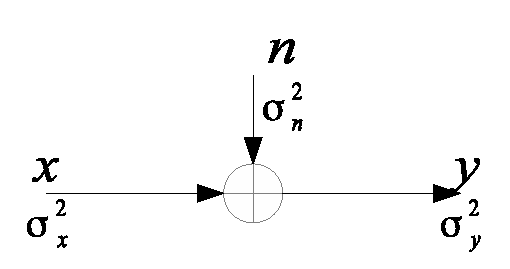
\includegraphics[width=0.25\textwidth]{AWGN_channel.eps} & C_{T}=B\ld\left(1+\frac{\sigma_{x}^{2}}{\sigma_{n}^{2}}\right)\frac{\mathrm{bit}}{\mathrm{s}} \\
	\text{flat fading:}\qquad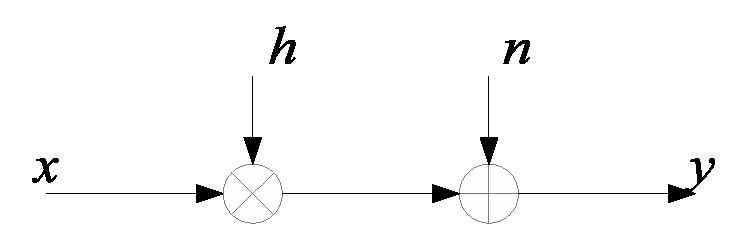
\includegraphics[width=0.3\textwidth]{flatfading_channel.eps} & C_{T}=B\ld\left(1+\frac{h^{2}\sigma_{x}^{2}}{\sigma_{n}^{2}}\right) \\
	\text{frequency selective:}\qquad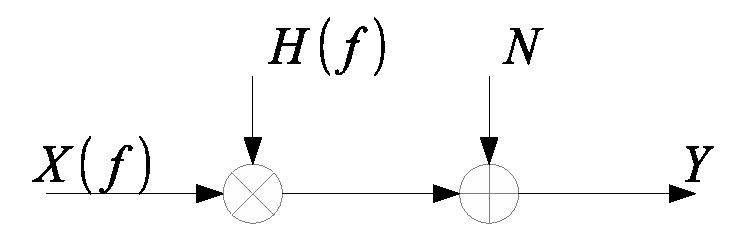
\includegraphics[width=0.3\textwidth]{frequencyselective_channel.eps} & \\
	\end{cases}& \\
	&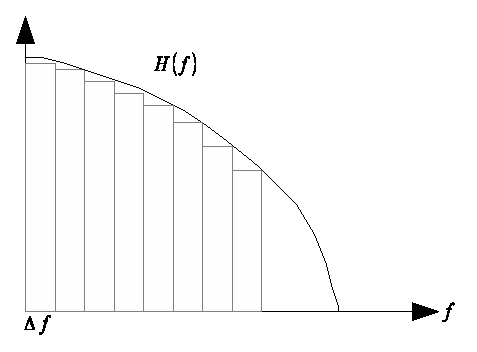
\includegraphics[width=0.5\textwidth]{frequencyselective_channel_2.eps}& \\
	&H_{i}\left(f\right)=\mathrm{const.}\quad\rightarrow\quad\text{Water-filling algorithm}& \\
	&\quad\qquad\qquad\qquad\rightarrow\quad\text{Allocate more power to better (with highter SNR) channels}& \\
	&\mathrm{dB}
	\begin{cases}
	\text{comparison: power $P_{1}$, $P_{2}\quad\rightarrow\quad P_{2}$ has $10\log\frac{P_{2}}{P_{1}}\mathrm{dB}$ more power than $P_{1}$} \\
	\text{absolute power: $\mathrm{dBm}$, $P_{2}=10\mathrm{W},\quad P_{1}=1\mathrm{W}\quad\rightarrow\quad P_{2}=10\log 10=10\mathrm{dB}$}
	\end{cases}& \\
	&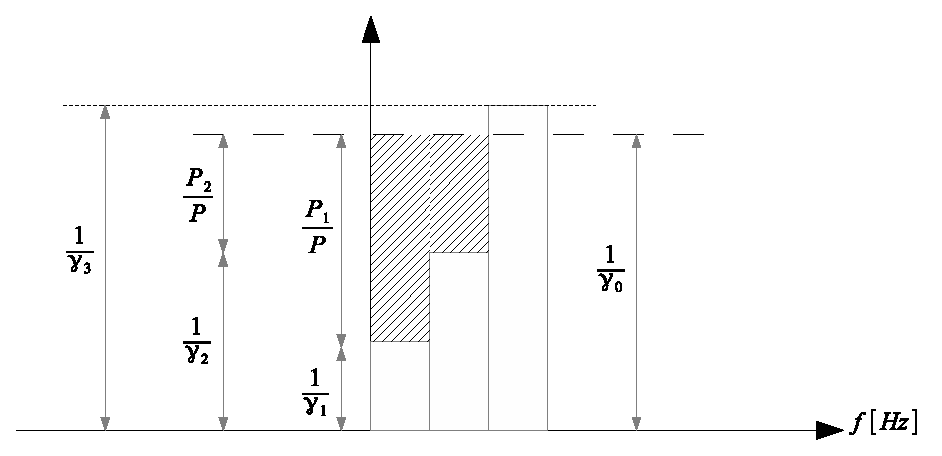
\includegraphics[width=1\textwidth]{waterfilling.eps}& \\
\end{align*}
\begin{align*}
	&\gamma_{i}=\text{SNR of $i$th channel}& \\
	&P_{i}=\text{allocated power to the $i$th channel}& \\
	&\frac{P_{i}}{P}=
	\begin{cases}
	\frac{1}{\gamma_{0}}-\frac{1}{\gamma_{i}} & \frac{\left|H_{i}\right|^{2}P}{\sigma_{n}^{2}}=\frac{\left|H_{i}\right|^{2}P}{N_{0}B}\ge\gamma_{0} \\
	0 & \text{otherwise}
	\end{cases}& \\
	&\sigma_{n}^{2}=N_{0}B\quad\text{with noise power $\sigma_{n}^{2}$ and PSD of noise $N_{0}$}& \\
	&H_{i}=\text{transfer function (channel gain) of $i$th channel}& \\
	&\text{Constraint:}\quad\sum_{i=1}^{3}P_{i}=P\quad\text{total transmit power}& \\
	&\sum_{i=1}^{3}P_{i}=P\quad\rightarrow\quad\sum_{i=1}^{3}\left(\frac{1}{\gamma_{0}}-\frac{1}{\gamma_{i}}\right)P=P\quad\rightarrow\quad\boxed{\sum_{i=1}^{3}\left(\frac{1}{\gamma_{0}}-\frac{1}{\gamma_{i}}\right)P=1}& \\
	&\gamma_{1}=\frac{\left|H_{1}\right|^{2}P}{N_{0}B}=\frac{1\cdot 10^{-3}}{10^{-11}\cdot 1ß^{7}}\quad\rightarrow\quad\gamma_{1}=10\quad\rightarrow\quad\text{best channel}& \\
	&\gamma_{2}=\frac{\left|H_{2}\right|^{2}P}{N_{0}B}=10H_{2}^{2}\quad\rightarrow\quad\gamma_{2}=2,5& \\
	&\gamma_{3}=\frac{\left|H_{3}\right|^{2}P}{N_{0}B}=10H_{3}^{2}\quad\rightarrow\quad\gamma_{3}=0,9\quad\rightarrow\quad\text{worst channel}& \\
	&\sum_{i=1}^{3}\left(\frac{1}{\gamma_{0}}-\frac{1}{\gamma_{i}}\right)=1\quad\Rightarrow\quad\frac{3}{\gamma_{0}}=1+\frac{1}{\gamma_{1}}+\frac{1}{\gamma_{2}}+\frac{1}{\gamma_{3}}\quad\rightarrow\quad\gamma_{0}=1,15\quad\text{(water level)}& \\
	&\qquad\rightarrow\text{water level check}\quad\rightarrow\quad\gamma_{i}>\gamma_{0}\forall i& \\
	&\gamma_{1}=10>\gamma_{0}\quad\checkmark& \\
	&\gamma_{2}=2,5>\gamma_{0}\quad\checkmark& \\
	&\gamma_{3}=0,9<\gamma_{0}\quad\lightning\quad\rightarrow\quad\text{no power can be allocated to channel 3}& \\
	&\sum_{i=1}^{2}\left(\frac{1}{\gamma_{0}}-\frac{1}{\gamma_{i}}\right)=1\quad\rightarrow\quad\frac{2}{\gamma_{0}}=1+\frac{1}{10}+\frac{1}{2,5}\quad\rightarrow\quad\gamma_{0}=1,33& \\
	&\gamma_{1}=10>\gamma_{0}\quad\checkmark& \\
	&\gamma_{2}=2,5>\gamma_{0}\quad\checkmark& \\
	&\quad\rightarrow\quad C_{\mathrm{T}}=B\sum\limits_{i=1}^{2}\ld\left(1+\frac{\left|H_{1}\right|^{i}P}{N_{0}B}\right)=B\sum\limits_{i=1}^{2}\ld\left(1+\frac{\gamma_{i}}{\gamma_{0}}-1\right)=B\sum\limits_{i=1}^{2}\ld\left(\frac{\gamma_{i}}{\gamma_{0}}\right)& \\
	&\qquad C_{\mathrm{T}}=10^{7}\left(\ld\left(\frac{10}{1,33}\right)+\ld\left(\frac{2,5}{1,33}\right)\right)\quad\rightarrow\quad C_{\mathrm{T}}=38,2\text{ Mbits/s}& \\
	&\qquad C_{\mathrm{T}}=B\ld\left(1+\frac{S}{N}\right)\quad\text{Shannon formula}& \\
\end{align*}
\section*{Problem 4}
\begin{align*}
	&\text{Multiplexing gain}\qquad\qquad G_{\mathrm{m}}=\lim_{\mathrm{SNR}\rightarrow\infty}\frac{R}{\ld\left(\mathrm{SNR}\right)}& \\
	&\text{Diversity gain}\quad\qquad\qquad C=\ld\left(1+\mathrm{SNR}\right)\quad\Rightarrow\quad C\overset{\mathrm{SNR}\rightarrow\infty}{\approx}\ld\left(\mathrm{SNR}\right)& \\
	&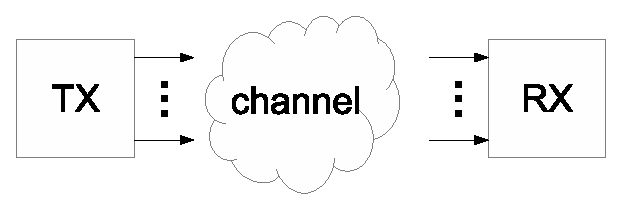
\includegraphics[width=0.7\textwidth]{MIMO_channel.eps}& \\
	&\text{Multiplexing gain $=$ number of parallel independent equivalent channels}& \\
	&\svd\left(H\right)\quad\rightarrow\quad\text{singular values of $H$: $\sigma_{i}^{2}$, $i\in\{1,2,\ldots,\rank\left(H\right)\}$}& \\
	&\rank\left(H\right)\quad\rightarrow\quad\text{number of singular values}& \\
	&H_{1}=
	\begin{bmatrix}
	1 & 1 & -1 \\
	-1 & 1 & 1 \\
	-1 & -1 & 1
	\end{bmatrix}\quad\rightarrow\quad\rank\left(H_{1}\right)=2& \\
	&\text{Matlab/Octave}\quad\rightarrow\quad\svd\left(H_{1}\right)=\mathbf{U}_{1}\mathbf{\Sigma}_{1}\mathbf{V}_{1}^{H}& \\
	&\qquad\mathbf{\Sigma}_{1}=
	\begin{bmatrix}
	2,56 & 0 & 0 \\
	0 & 1,56 & 0 \\
	0 & 0 & 0 
	\end{bmatrix}\quad\rightarrow\quad\text{$\sigma_{1}=2,56$, $\sigma_{2}=1,56$, $\sigma_{3}=0$ $\rightarrow$ useless}& \\
	&H_{2}=
	\begin{bmatrix}
	1 & -1 & -1 \\
	-1 & -1 & 1 \\
	1 & -1 & 1
	\end{bmatrix}\quad\rightarrow\quad\rank\left(H_{2}\right)=3\quad\rightarrow\quad\text{full rank}& \\
	&\svd\left(H_{1}\right)=\mathbf{U}_{2}\mathbf{\Sigma}_{2}\mathbf{V}_{2}^{H}& \\
	&\qquad\mathbf{\Sigma}_{2}=
	\begin{bmatrix}
	2 & 0 & 0 \\
	0 & 2 & 0 \\
	0 & 0 & 1 
	\end{bmatrix}\quad\rightarrow\quad\text{$\sigma_{1}=2$, $\sigma_{2}=2$, $\sigma_{3}=1$}& \\
\end{align*}
\section*{Problem 5}
\begin{align*}
	&\text{MIMO channel capacity}& \\ 
	&\text{short review:}& \\
	&\text{1 - channel matrix is deterministic and known to the transmitter}& \\
	&\text{2 - channel matrix is random and changes during the transmission of a code word}& \\
	&\qquad\text{$\rightarrow$ ergodic capacity}& \\
	&\text{3 - channel matrix is random and fixed during the transmission of a code word,}& \\ 
	&\qquad\text{but only known to TX}& \\
	&\text{Decompose the MIMO channel to subchannels}& \\
	&C_{\mathrm{T}}=B\sum_{i=1}^{N}\left[\ld\underbrace{\left(\frac{x_{i}^{2}}{\sigma_{n}^{2}}\mu\right)}_{\substack{\text{equivalent SNR} \\ \text{of channel $i$}}}\right]& \\
	&\qquad B:\quad\text{Bandwidth}& \\
	&\qquad x_{i}:\quad\text{singular value of H}& \\
	&\qquad\sigma_{n}^{2}:\quad\text{noise power}& \\
	&\qquad\mu :\quad\text{water level}& \\
	&\svd\left(\mathbf{H}\right)=\svd\left(
	\begin{bmatrix}
	0,2 & -0,2 & 0,2 \\
	0,1 & 0,4 & -1 \\
	1 & 0,2 & 1
	\end{bmatrix}\right)=\mathbf{U\Sigma V}^{H}& \\
	&\qquad\mathbf{\Sigma}=
	\begin{bmatrix}
	1,61 & 0 & 0 \\
	0 & 0,82 & 0 \\
	0 & 0 & 0,2
	\end{bmatrix}\quad\rightarrow\quad
	\begin{matrix}
	x_{1} = 1,61 \\
	x_{2} = 0,82 \\
	x_{3} = 0,2
	\end{matrix}& \\
	&\frac{P}{\sigma_{n}^{2}}=10\mathrm{dB}\quad\rightarrow\quad\frac{P}{\sigma_{n}^{2}}=10& \\
	&\gamma_{1}=x^{2}\frac{P}{\sigma_{n}^{2}}=1,61^{2}\cdot 10=25,9& \\
	&\gamma_{2}=0,82^{2}\cdot 10=7,6& \\
	&\gamma_{3}=0,2^{2}\cdot 10=0,4& \\
	&\qquad\text{3 non-zero singular values $\rightarrow$ number of parallel independent channels $=3$}& \\
	&\sum_{i=1}^{3}\left(\mu-\frac{1}{\gamma_{i}}\right)=1& \\
	&\qquad\rightarrow\quad 3\mu=\frac{1}{\gamma_{1}}+\frac{1}{\gamma_{2}}+\frac{1}{\gamma_{3}}+1=3,7\quad\rightarrow\quad\mu=1,23\quad\text{water level}&
\end{align*}
\begin{align*}
	&\text{water level check:}
	\begin{cases}
	\frac{1}{\gamma_{1}}=0,039<\mu\quad\checkmark \\
	\frac{1}{\gamma_{2}}=0,15<\mu\quad\checkmark \\
	\frac{1}{\gamma_{3}}=2,5>\mu \quad\lightning\quad\text{3rd channel doesn't have enough SNR}
	\end{cases}& \\
	&\qquad\Rightarrow\quad\text{no power can be allocated to 3rd channel}& \\
	&\qquad\Rightarrow\quad\text{allocate power in 1st and 2nd channel}& \\
	&\rightarrow\sum_{i=1}^{2}\left(\mu-\frac{1}{\gamma_{i}}\right)=1& \\
	&\rightarrow 2\mu=\frac{1}{\gamma_{1}}+\frac{1}{\gamma_{2}}+1=1,19\quad\rightarrow\quad\mu=0,595\quad\text{water level}& \\
	&\text{water level check:}
	\begin{cases}
	\frac{1}{\gamma_{1}}<\mu\quad\checkmark \\
	\frac{1}{\gamma_{2}}<\mu\quad\checkmark \\
	\end{cases}& \\
	&\rightarrow C_{\mathrm{T}}=B\sum_{i=1}^{2}\ld\left(\mu\gamma_{i}\right)=10^{6}\left(\ld\left(\frac{25,9}{0,595}\right)+\ld\left(\frac{6,7}{0,595}\right)\right)& \\
	&\rightarrow C_{\mathrm{T}}=8,937\text{ Mbit/s}& \\
	&\text{no CSIT: }& \\
	&\rightarrow C_{\mathrm{T}}=B\sum_{i=1}^{3}\ld\left(1+x_{i}^{2}\frac{P_{i}}{\sigma_{n}^{2}}\right)=B\sum_{i=1}^{3}\ld\left(1+x_{i}^{2}\frac{P}{3\sigma_{n}^{2}}\right)& \\
	&\rightarrow C_{\mathrm{T}}=10^{6}\left(\ld\left(1+8,64\right)+\ld\left(1+2,24\right)+\ld\left(1+0,13\right)\right)& \\
	&\rightarrow C_{\mathrm{T}}=5,14\text{ Mbit/s}& \\
	&\text{no CSIT at transmitter result in approx. $3,8$ Mbit/s data rate degradation}&
\end{align*}

\begin{align*}
&\text{Hier fehlen Aufgabe 6-7???}& \\
&\text{das folgende gehört zu Aufgabe 8 SISO Rayleigh fading channel}& \\
&\text{ACHTUNG: doppelte Nummerierung: Aufgabe 8 Receiver diversity, MRC, EGC and SC}&
\end{align*}

\section*{Problem 8.1\footnote[1]{Problem 8 kommt 2mal vor, sind aber unterschiedliche Aufgaben} - SISO Rayleigh fading channel}
\begin{align*}
	&\overline{\mathrm{SER}}=\mathbb{E}_{\left|h\right|^{2}}\left\{\mathrm{SER}\left(\left|h\right|^2\right)\right\}& \\
	& 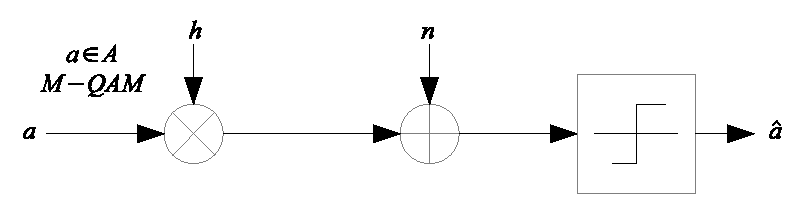
\includegraphics[width=0.6\textwidth]{rx_chain.eps} & \\
	&\mathrm{SER}\left(\left|h\right|^2\right)=C_{\mathcal{A}}\mathrm{Q}\left(\sqrt{d_\mathrm{min}^2\frac{E_{b}}{N_0}}\left|h\right|^2\right)& \\
	&\qquad C_{\mathcal{A}}=3\quad\left(\text{16-QAM}\right)\qquad\qquad C_{\mathcal{A}}=2\quad\left(\text{4-QAM}\right)& \\
	&\qquad =C_{\mathcal{A}}\mathrm{Q}\left(\sqrt{\underbrace{\frac{d_\mathrm{min}^2}{\ld(\left(M\right)}}_{d_{\mathcal{A}^2}} \underbrace{\frac{E_{s}}{N_0}}_{\gamma}\left|h\right|^2}\right)=C_{\mathcal{A}}\mathrm{Q}\left(\sqrt{d_\mathcal{A}^2\gamma\left|h\right|^2}\right)& \\
	&h\sim CN\left(0,1\right)\quad\rightarrow\quad\left|h\right|^2\text{ is exponentially distributed with variance 1}& \\
	&\quad\rightarrow\overline{\mathrm{SER}}=\int\limits_0^\infty \underbrace{f_{\left|h\right|^2}\left(x\right)}_{\text{pdf of }\left|h\right|^2} \mathrm{SER}\left(x\right)\mathrm{d}x=\int\limits_0^\infty\mathrm{e}^{-x}C_{\mathcal{A}}\mathrm{Q}\left(\sqrt{d_\mathcal{A}^2\gamma\left|h\right|^2}\right)\mathrm{d}x& \\
	&\qquad\mathrm{Q}\left(x\right)=\frac{1}{2\pi}\int\limits_x^\infty e^{-\frac{t^2}{2}}\mathrm{d}t& \\
	&\quad\rightarrow\quad\overline{\mathrm{SER}}=\int\limits_0^\infty e^{-x}C_\mathcal{A}\frac{1}{\sqrt{2\pi}}\int\limits_{\sqrt{d_\mathcal{A}^2\gamma_x}}^\infty e^{-\frac{t^2}{2}}\mathrm{d}t\,\mathrm{d}x& \\
	&\quad\rightarrow\quad\text{change the order of integrals}& \\
	&\quad\rightarrow\quad\overline{\mathrm{SER}}=\frac{C_\mathcal{A}}{\sqrt{2\pi}}\int\limits_{\sqrt{d_\mathcal{A}^2\gamma_x}}^\infty\int\limits_0^\infty e^{-x}e^{-\frac{t^2}{2}}\mathrm{d}x\,\mathrm{d}t&
\end{align*}
\begin{align*}
	& 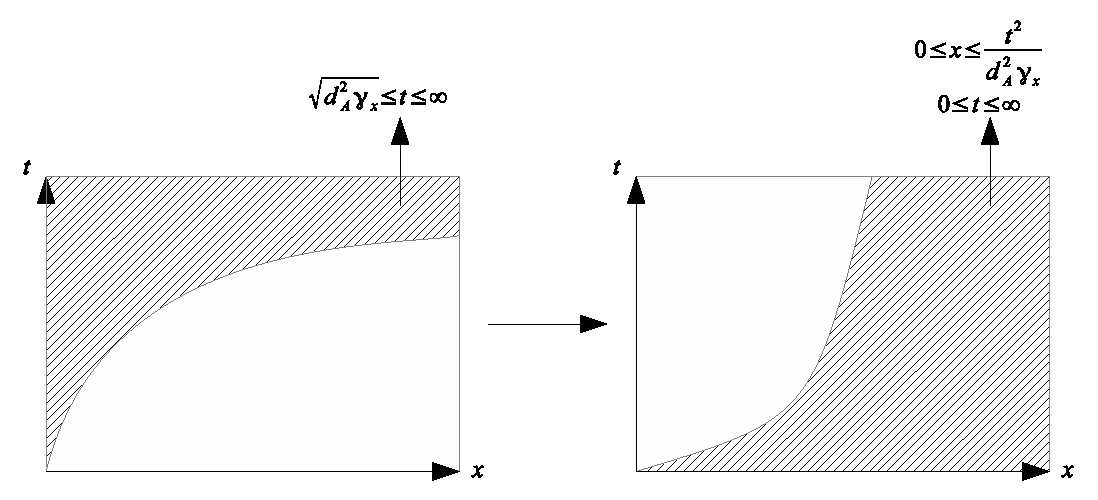
\includegraphics[width=1\textwidth]{integration.eps} & \\
	\overline{\mathrm{SER}} & =\frac{C_\mathcal{A}}{\sqrt{2\pi}}\int\limits_0^\infty\int\limits_0^\frac{t^2}{d_\mathcal{A}^2\gamma}e^{-x}e^{-\frac{t^2}{2}}\mathrm{d}x\,\mathrm{d}t=\frac{C_\mathcal{A}}{\sqrt{2\pi}}\int\limits_0^\infty e^{-\frac{t^2}{2}}\left[e^{-x}\right]_0^{\frac{t^2}{d_\mathcal{A}^2\gamma}}\mathrm{d}t= \\
	& =\frac{C_\mathcal{A}}{\sqrt{2\pi}}\int\limits_0^\infty e^{-\frac{t^2}{2}}\left(-e^{-\frac{t^2}{d_\mathcal{A}^2\gamma}}+1\right)\mathrm{d}t= \\
	& =\frac{C_\mathcal{A}}{\sqrt{2\pi}}\int\limits_0^\infty\left(e^{-\frac{t^2}{2}}-e^{-\frac{t^2}{2}\left(1+\frac{2}{d_\mathcal{A}^2\gamma}\right)}\right)\mathrm{d}t= \\
	& =\frac{C_\mathcal{A}}{\sqrt{2\pi}}\left(\sqrt{2\pi}\underbrace{\mathrm{Q}\left(0\right)}_{\frac{1}{2}}-\sqrt{\frac{2\pi}{1+\frac{2}{d_\mathcal{A}^2\gamma}}}\underbrace{\mathrm{Q}\left(\sqrt{1+\frac{2}{d_\mathcal{A}^2\gamma}}0\right)}_{0}\right)= \\
	& =\frac{C_\mathcal{A}}{2}\left(1-\sqrt{\frac{1}{1+\frac{2}{d_\mathcal{A}^2\gamma}}}\right)=\boxed{\frac{C_\mathcal{A}}{2}\left(1-\sqrt{\frac{d_\mathcal{A}^2\gamma}{d_\mathcal{A}^2\gamma+2}}\right)} \\
\end{align*}

\subsection*{d)}
\begin{align*}
	& \text{Asymptotic $\overline{\mathrm{SER}}$ if $\gamma\rightarrow\infty$} \\
	& \overline{\mathrm{SER}}=\frac{C_\mathcal{A}}{2}\left(1-\sqrt{\frac{d_\mathcal{A}^2\gamma}{d_\mathcal{A}^2\gamma+2}}\right) \\
	& \qquad C_\mathcal{A}:\text{ average number of nearest neighbours in the constellation diagram} \\
	& \text{Taylor series:}\quad f\left(x\right)\approx f\left(x_0\right)+\left(x-x_0\right)f'\left(x_0\right)+\frac{\left(x-x_0\right)^2}{2}f''\left(x_0\right)+\ldots \\
	& \text{uppper bound:}\quad f\left(x\right)\approx f\left(x_0\right)+\left(x-x_0\right)f'\left(x_0\right) \\
	& \quad x_0=0\quad\rightarrow\quad f\left(x\right)=f\left(0\right)+xf'\left(0\right) \\
	& \quad x=\frac{1}{d_\mathcal{A}^2\gamma}\text{ if }\gamma\rightarrow\infty\quad\Rightarrow\quad x=0 \\
	& \overline{\mathrm{SER}}\left(x\right)=\frac{C_\mathcal{A}}{2}\left(1-\sqrt{\frac{1}{1+2x}}\right) \\
	& \overline{\mathrm{SER}}\left(x\right)\le\overline{\mathrm{SER}}\left(0\right)+x\mathrm{SER}'\left(0\right) \\
	& \quad\overline{\mathrm{SER}}\left(0\right)=\frac{C_\mathcal{A}}{2}\left(1-\sqrt{\frac{1}{1}}\right)=0 \\
	& \quad\overline{\mathrm{SER}'}\left(x\right)=-\frac{C_\mathcal{A}}{2}\frac{1}{2\sqrt{\frac{1}{1+2x}}}\frac{-1}{\left(1+2x\right)^2}2\quad\Rightarrow\quad\overline{\mathrm{SER}'}\left(0\right)=-\frac{C_\mathcal{A}}{2} \\
	& \quad\rightarrow\quad\overline{\mathrm{SER}}\left(x\right)\le\frac{C_\mathcal{A}}{2}x\quad\rightarrow\quad\boxed{\overline{\mathrm{SER}}\left(\gamma\right)\le\frac{C_\mathcal{A}}{2}\frac{1}{d_\mathcal{A}^2\gamma}} \\
	& \mathrm{SER}\left(\left|h\right|^2\right)=C_\mathcal{A}\mathrm{Q}\left(\sqrt{d_\mathcal{A}^2\gamma\|h\|^2}\right) \\
	& \qquad\text{we could have used Chernoff bound: }\mathrm{Q}\left(x\right)\le\frac{1}{2}\mathrm{e}^{-\frac{x^2}{2}} \\
	& \mathrm{SER}\left(\left|h\right|^2\right)\le\frac{C_\mathcal{A}}{2}e^{-\frac{d_\mathcal{A}^2\|h\|^2\gamma}{2}}\quad\rightarrow\quad\ldots\quad\rightarrow\quad\boxed{\overline{\mathrm{SER}}\le C_\mathcal{A}\frac{1}{d_\mathcal{A}^2\gamma}} \\
\end{align*}
\section*{Problem 8.2 - Receiver diversity, MRC, EGC and SC}
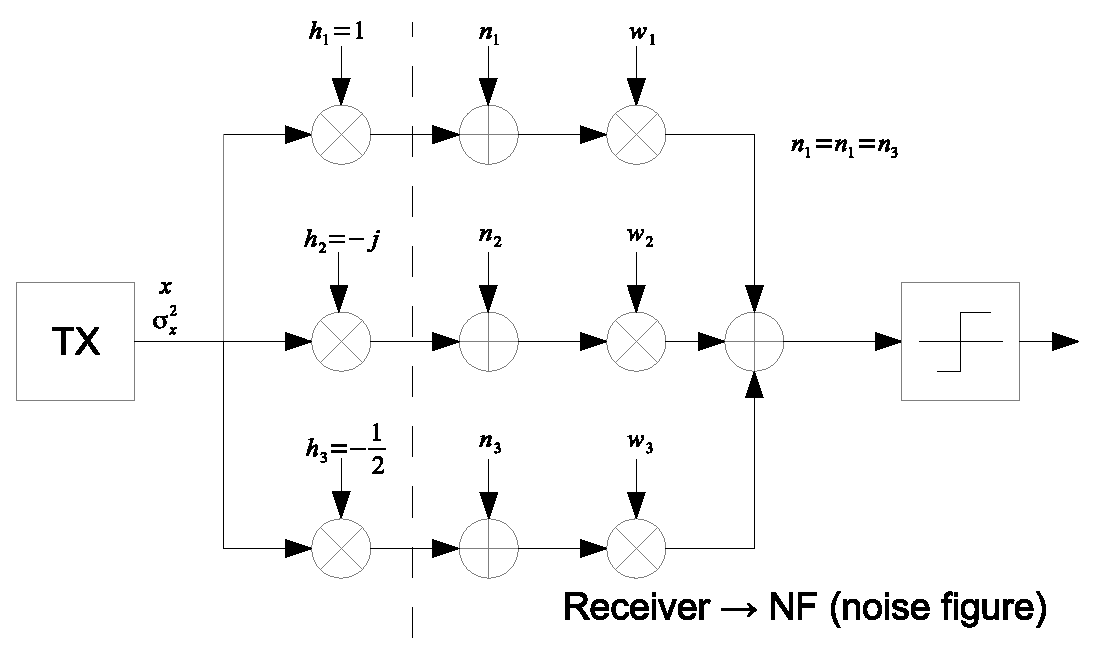
\includegraphics[width=1\textwidth]{MIMO_receiver.eps} \\
\subsection*{a)}
\begin{align*}
	\mathrm{MRC}\quad\rightarrow\quad & w_j =h_j^*\quad\forall j\in\{1,\ldots,N_R\} \\
	& w_1=1 \\
	& w_2=j \\
	& w_3=-\frac{1}{2} \\
	&\text{In order to have $w_j$ we need $h_j$ $\rightarrow$ channel estimation} \\
	\mathrm{EGC}\quad\rightarrow\quad & h_n=\left|h_n\right|e^{j\phi_n}\quad\Rightarrow\quad w_n=e^{j\phi_n} \\
	& h_1=1\quad\rightarrow\quad w_1=1 \\
	& h_2=-j\quad\rightarrow\quad w_2=j \\
	& h_3=-\frac{1}{2}\quad\rightarrow\quad w_3=e^{-j\pi}=-1
\end{align*}

\subsection*{b)}
\begin{align*}
	\mathrm{MRC:} & \quad\mathrm{SNR_{total}^{MRC}}=\frac{\sigma_x^2\left|\sum\limits_{n=1}^{N_R}h_nw_n\right|^2}{\sigma_n^2\sum\limits_{n=1}^{N_R}\left|w_n\right|^2} = \frac{\sigma_x^2\left|\sum\limits_{n=1}^{N_R}\left|h_n\right|e^{j\phi_n}\left|h_n\right|e^{-j\phi_n}\right|^2}{\sigma_n^2\sum\limits_{n=1}^{N_R}\left|h_n\right|^2}= \\
	& \qquad=\frac{\sigma_x^2}{\sigma_n^2}\left(\sum\limits_{n=1}^{N_R}\left|h_n\right|^2\right)=\frac{\sigma_x^2}{\sigma_n^2}\left(1+1+\frac{1}{4}\right) \\
	& \qquad\Rightarrow\boxed{\mathrm{SNR_{total}^{MRC}}=\frac{9}{4}\frac{\sigma_x^2}{\sigma_n^2}} \\
	\mathrm{EGC:} & \quad\mathrm{SNR_{total}^{EGC}}=\frac{\sigma_x^2\left|\sum\limits_{n=1}^{N_R}\left|h_n\right|e^{j\phi_n}e^{-j\phi_n}\right|^2}{\sigma_n^2\sum\limits_{n=1}^{N_R}\left|e^{-j\phi_n}\right|^2}= \\
	& \qquad=\frac{\sigma_x^2}{N_R\sigma_n^2}\left(\sum\limits_{n=1}^{N_R}\left|h_n\right|^2\right)=\frac{\sigma_x^2}{3\sigma_n^2}\left(1+1+\frac{1}{2}\right)^2 \\
	& \qquad\Rightarrow\boxed{\mathrm{SNR_{total}^{EGC}}=\frac{25}{12}\frac{\sigma_x^2}{\sigma_n^2}} \\
	\mathrm{SC:} & \quad\text{branch with max. SNR: } \hat{n}=\argmax_n\mathrm{SNR}_n\quad\rightarrow\quad\mathrm{SNR_{total}}=\mathrm{SNR}_{\hat{n}} \\
	& \quad\text{we need SNR estimation algorithm $\rightarrow$ e.g. pilots} \\
	& \qquad\mathrm{SNR}_1=\frac{\sigma_x^2\left|h_1\right|^2\left|w_1\right|^2}{\sigma_n^2\left|w_1\right|^2}=\frac{\sigma_x^2}{\sigma_n^2}\left|h_1\right|^2=\frac{\sigma_x^2}{\sigma_n^2} \\
	& \qquad\mathrm{SNR}_2=\frac{\sigma_x^2}{\sigma_n^2}\left|h_2\right|^2=\frac{\sigma_x^2}{\sigma_n^2} \\
	& \qquad\mathrm{SNR}_3=\frac{\sigma_x^2}{\sigma_n^2}\left|h_3\right|^2=\frac{1}{4}\frac{\sigma_x^2}{\sigma_n^2} \\
	& \quad\text{$\mathrm{SNR}_1$/$\mathrm{SNR}_2$ is the highest SNR, we select first branch} \\
	& \quad\rightarrow\quad\boxed{\mathrm{SNR_{total}^{SC}}=\mathrm{SNR}_1=\frac{\sigma_x^2}{\sigma_n^2}}
\end{align*}
\begin{align*}
	\left.
	\begin{aligned}
		\mathrm{MRC:} & \quad\mathrm{SNR_{total}^{MRC}}=\frac{4}{9}\frac{\sigma_x^2}{\sigma_n^2} \\
    \mathrm{EGC:} & \quad\mathrm{SNR_{total}^{EGC}}=\frac{25}{12}\frac{\sigma_x^2}{\sigma_n^2} \\
		\mathrm{SC:} & \quad\mathrm{SNR_{total}^{SC}}=\frac{\sigma_x^2}{\sigma_n^2}
  \end{aligned}
	\right\}
	\quad\boxed{\mathrm{SNR}^{MRC}\ge\mathrm{SNR}^{EGC}\ge\mathrm{SNR}^{SC}}
\end{align*}

\section*{Problem 9 - BPSK error rate in an MRC system over Nakagami-m channel}
\begin{align*}
	& \text{SNR distribution for Nakagami-m fading}\\
	& \mathrm{pdf:}\quad P_\gamma\left(x\right)=\frac{m^mx^{m-1}}{\gamma^{-m}\Gamma\left(m\right)}\mathrm{exp}\left(-\frac{mx}{\bar{\gamma}}\right)
	\begin{cases}
		m & \text{fading parameter} \\
		\Gamma\left(m\right) & \text{Gamma function }=(m-1)! \\
		\bar{\gamma} & \text{average branch SNR}
	\end{cases} \\
	&\rightarrow\text{Laplace transform} \\
	&\mathcal{L}\left(P_\gamma\left(x\right)\right)=M_\gamma\left(s\right)\quad\rightarrow\quad\text{moment generating function (mgs)} \\
	&\rightarrow M_\gamma\left(s\right)=\left(1-\frac{s\bar{\gamma}}{m}\right)^{-m}\quad m=1\quad\Rightarrow\quad\text{Rayleigh} \\
	&\gamma_\mathrm{total}^\mathrm{MRC}=\sum\limits_{n=1}^{N_R}\gamma_n\qquad\gamma_n:\text{ branch SNR} \\
	&\text{Probability density function pdf of total SNR is convolution of branch SNR.} \\
	&\text{Convolution in time domain $\rightarrow$ multiplication in frequency domain.} \\
	&\text{i.i.d fading $\rightarrow$ branch SNR independent} \\
	&\quad\rightarrow M_{\gamma_\mathrm{total}}\left(s\right)=\prod\limits_{n=1}^{N_R}M_{\gamma_n}\left(s\right)=\left(M_\gamma\left(s\right)\right)^{N_R} \\
	&\quad\rightarrow M_{\gamma_\mathrm{total}}\left(s\right)=\left(1-\frac{s\bar{\gamma}}{m}\right)^{-mN_R} \\
	&\text{from lecture notes:} \\
	&\rightarrow \bar{P}_e=\frac{a}{\pi}\int\limits_0^{\frac{\pi}{2}}{M_\gamma}_\mathrm{total}\left(\frac{b}{2\sin^2\Theta}\right)\mathrm{d}\Theta \\
	&\text{$a$, $b$ are parameters depending on modulation scheme} \\
	&\rightarrow\text{for BPSK: $a=1$, $b=2$} \\
	&\rightarrow\quad\boxed{\bar{P}_e=\frac{1}{\pi}\int\limits_0^{\frac{\pi}{2}}\left(1-\frac{\bar{\gamma}}{m\sin^2\Theta}\right)^{-mN_R}\mathrm{d}\Theta}
\end{align*}
\section*{Problem 10 - MPSK error rate in an MRC system over a mixed Rayleigh, Nakagami-m channel}
\begin{align*}
	&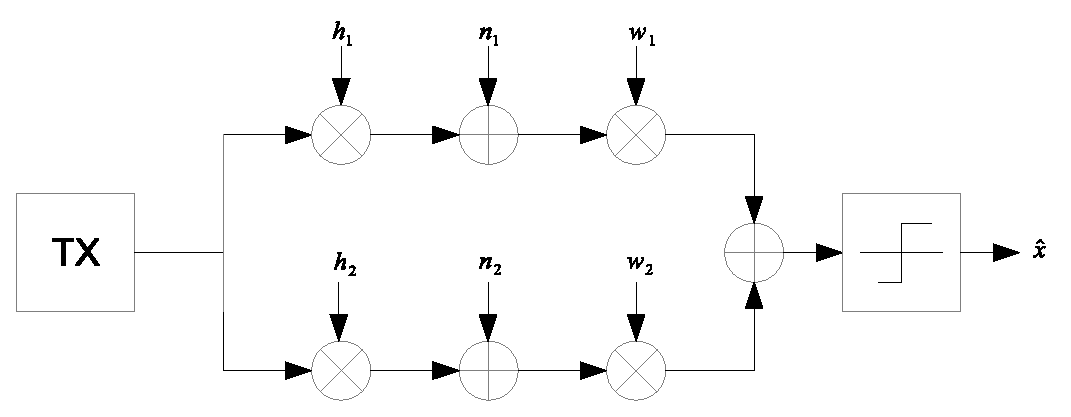
\includegraphics[width=1\textwidth]{MIMO_receiver_2.eps} \\
	&{\sigma_n^2}_1={\sigma_n^2}_2={\sigma_n^2}_1 \\
	&\text{branch SNR: }\bar{\gamma}=\frac{\sigma_x^2}{\sigma_n^2} \\
	&\text{branch 1}\quad\rightarrow\quad\text{Rayleigh}\quad\rightarrow\quad p_\gamma\left(x\right)=\frac{1}{\bar{\gamma}}\mathrm{exp}\left(\frac{x}{\bar{\gamma}}\right) \\
	&\text{branch 2}\quad\rightarrow\quad\text{Nakagami-m}\quad\rightarrow\quad p_\gamma\left(x\right)=\frac{m^mx^{m-1}}{\gamma^{-m}\Gamma\left(m\right)}\mathrm{exp}\left(-\frac{mx}{\bar{\gamma}}\right) \\
	&\text{i.i.d fading}\quad\rightarrow\quad {M_\gamma}_\mathrm{total}\left(s\right)={M_\gamma}_1\left(s\right){M_\gamma}_2\left(s\right) \\
	&\begin{cases}
		\quad\text{first branch}\quad\rightarrow\quad\text{Rayleigh}\quad\rightarrow\quad{M_\gamma}_1\left(s\right)=\left(1-s\bar{\gamma}\right)^{-1} \\
		\quad\text{second branch}\quad\rightarrow\quad\text{Nakagami-m}\quad\rightarrow\quad{M_\gamma}_2\left(s\right)=\left(1-\frac{s\bar{\gamma}}{m}\right)^{-m} \\
	\end{cases} \\
	&\quad\rightarrow\quad{M_\gamma}_\mathrm{total}=\left(1-s\bar{\gamma}\right)^{-1}\left(1-s\frac{\bar{\gamma}}{m}\right)^{-m} \\
	&\text{from lectures notes:} \\
	&\rightarrow\bar{P}_e=\int_0^\infty P_e{p_\gamma}_\mathrm{total}\left(x\right)\mathrm{d}x = \\ 
	&\qquad=\int\limits_0^\infty\frac{1}{\pi}\int\limits_0^{\frac{\left(M-1\right)\pi}{M}}\mathrm{exp}\left(\right)\mathrm{d}\Theta\,{p_\gamma}_\mathrm{total}\left(x\right)\mathrm{d}x= \\
	&\qquad=\frac{1}{\pi}\int\limits_0^{\frac{\left(M-1\right)\pi}{M}}\int\limits_0^\infty\mathrm{exp}\left(\frac{-x\sin^2\left(\frac{\pi}{M}\right)}{\sin^2\Theta}\right){p_\gamma}_\mathrm{total}\left(x\right)\mathrm{d}x\,\mathrm{d}\Theta= \\
	&\qquad=\int\limits_0^\infty e^{sx}{p_\gamma}_\mathrm{total}\left(x\right)\mathrm{d}x={M_\gamma}_\mathrm{total}\left(s\right)
\end{align*}
\begin{align*}
	&\rightarrow\int\limits_0^\infty\mathrm{exp}\left(\frac{-x\sin^2\left(\frac{\pi}{M}\right)}{\sin^2\Theta}\right){p_\gamma}_\mathrm{total}\left(x\right)\mathrm{d}x={M_\gamma}_\mathrm{total}\left(\frac{-\sin^2\left(\frac{\pi}{M}\right)}{\sin^2\Theta}\right) \\
	&\rightarrow\bar{p}_e=\frac{1}{M}\int\limits_0^{\frac{\left(M-1\right)\pi}{M}}{M_\gamma}_\mathrm{total}\left(\frac{-\sin^2\left(\frac{\pi}{M}\right)}{\sin^2\Theta}\right)\mathrm{d}\Theta \\
	&\rightarrow\boxed{\bar{p}_e=\frac{1}{M}\int\limits_0^{\frac{\left(M-1\right)\pi}{M}}\left(1+\frac{\bar{\gamma}\sin^2\left(\frac{\pi}{M}\right)}{\sin^2\Theta}\right)^{-1}\left(1+\frac{\bar{\gamma}\sin^2\left(\frac{\pi}{M}\right)}{m\sin^2\Theta}\right)^{-m}\mathrm{d}\Theta} \\
	&\bar{\gamma}=10\,\mathrm{dB}\qquad M=8\rightarrow 8\mathrm{PSK}\qquad m=3\qquad\Rightarrow\quad\bar{p}_e=0,0476
\end{align*}
\section*{Problem 11 - Transmit and receive diversity}
\begin{align*}
	& \text{The standard definition of outage probability:} \\
	& \quad\text{The average rate is \uline{lower} than a specific value.} \\
	& \text{Alternative definition:} \\
	& \quad\text{The error rate \uline{exceeds} a specific value.} \\
	& P_b=10^{-4}\quad\&\quad\text{BPSK modulation} \\
	& \quad\rightarrow\quad P_b\left(\gamma_0\right)=\mathrm{Q}\left(\sqrt{2\gamma_0}\right) \\
	& \quad\rightarrow\quad 10^{-4}=\mathrm{Q}\left(\sqrt{2\gamma_0}\right)\quad\rightarrow\quad\gamma_0=\frac{1}{2}\left(\mathrm{Q_{???}}\left(10^{-4}\right)\right)^2 \\
	& \quad\rightarrow\quad\gamma_0=6,9155\quad\rightarrow\quad\gamma_0=8,4\,\mathrm{dB} \\
	& \quad\rightarrow\quad P_{out}=P_e\left(\gamma_{total}<\gamma_0\right)=P\left(\gamma_{out}<6,9155\right) \\
	& \text{from lecture notes:} \\
	& \quad\rightarrow\quad{p_\gamma}_{total}\left(x\right)=\frac{x^{N_R-1}e^{-\frac{\lambda}{\bar{\gamma}}}}{\gamma^{-N_R}\left(N_R-1\right)!} \\
	& \quad\text{pdf of total SNR from MRC with i.i.d Rayleigh} \\
	& \rightarrow P_{out}=P_e\left(\gamma_{total}<6,9155\right)=\int\limits_0^{6,9155}\frac{x^{N_R-1}e^{-\frac{\lambda}{\bar{\gamma}}}}{\gamma^{-N_R}\left(N_R-1\right)!}\mathrm{d}x= \\
	& \qquad=1-e^{-\frac{6,9155}{10}}\sum\limits_{k=1}^3\frac{\left(\frac{6,9155}{10}\right)^{k-1}}{\left(k-1\right)!}=0,033=3,3\% \\
	& \qquad\bar{\gamma}=10\qquad N_R=3
\end{align*}
\section*{Problem 12 - Linear and decision-feedback MIMO detection}
\begin{align*}
	& \text{\uline{MIMO-MRC}} \\
	& \sigma_{n_1}^2=\sigma_{n_2}^2=\ldots=\sigma_{N_R}^2=\sigma_n^2 \\
	& 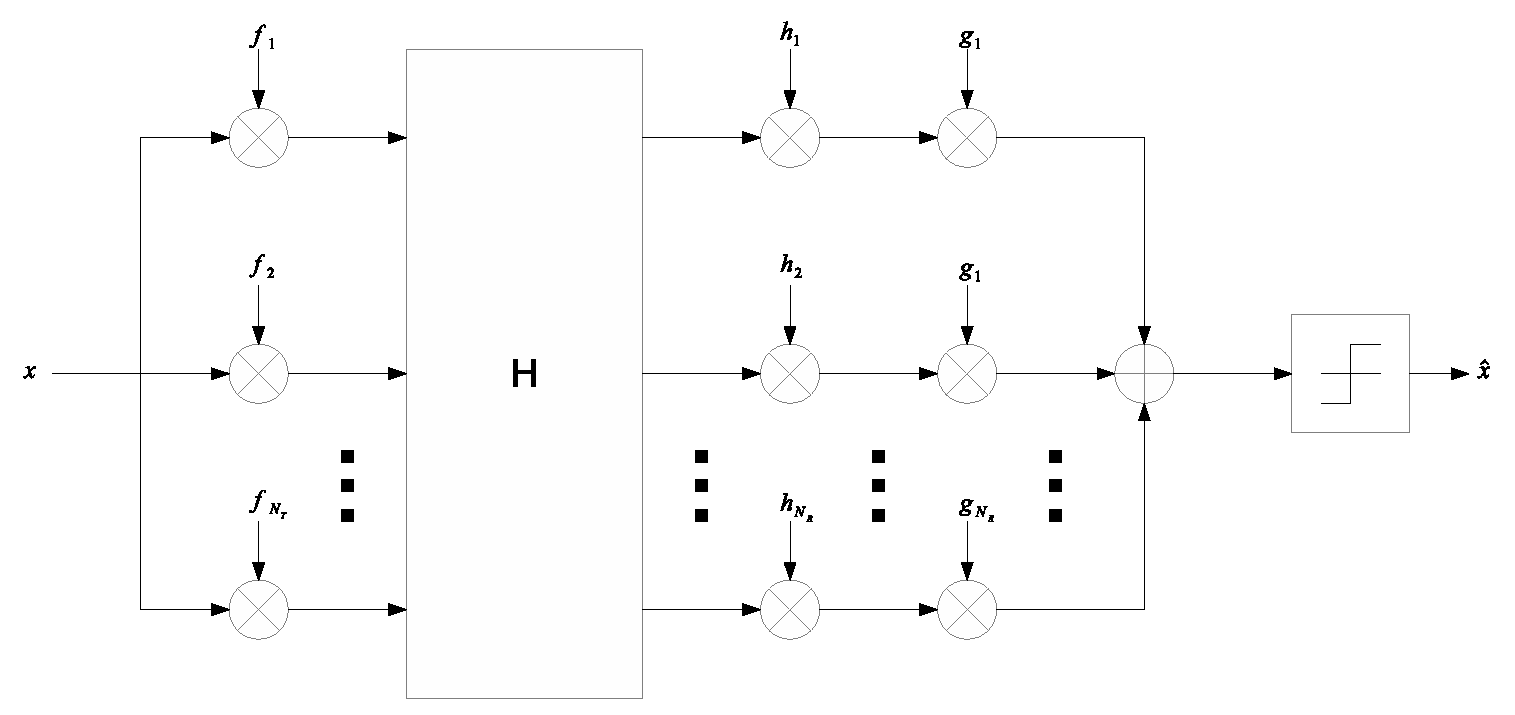
\includegraphics[width=1\textwidth]{MIMO_MRC.eps} \\
	& f=\left(f_1,f_2,\ldots,f_{N_R}\right)^T;\qquad g=\left(g_1^*,g_2^*,\ldots,g_{N_R}^*\right) \\
	& \quad\rightarrow\quad\text{Nomenclature:}\quad
	\begin{cases}
	f^Hf=1=\|f\|^2 \\
	g^Hg=1=\|g\|^2
	\end{cases} \\
	& \text{singular value decomposition:}\quad\mathbf{H=U\Sigma V}^H \\
	& \mathbf{\Sigma} =\diag\left(\xi_1^2,\xi_2^2,\ldots,\xi_N^2\right) \\
	& \quad\rightarrow\quad\text{sorted in descending order}\quad\rightarrow\quad\xi_1^2=\xi_{max}^2 \\
	& f = \mathbf{V}f'\quad\rightarrow\quad\mathbf{V}^Hf=\underbrace{\mathbf{V}^H\mathbf{V}}_{\mathbf{I}}f'=f'\quad\rightarrow\quad\|f'\|^2=\|\mathbf{V}^Hf\|^2\overset{\mathbf{V}: unitary}{=}\|f\|^2=1 \\
	& \text{in a similar way:} \\
	& \quad\rightarrow\quad g=u\cdot g' \\
	& \quad\rightarrow\quad \|g\|^2=\|g'\|^2=1 \\
	& \mathrm{SNR}=\frac{\sigma_x^2\left|\overbrace{h_{total}}^{\substack{\text{total transfer} \\ \text{function}}}\right|^2}{\sigma_n^2\underbrace{\|g\|^2}_{\rightarrow =1}}= \frac{\sigma_x^2\left|g^HHf\right|}{\sigma_n^2}=\frac{\sigma_x^2\left|g'^H\mathbf{U}^H\mathbf{U\Sigma V}^H\mathbf{V}f'\right|}{\sigma_n^2} \\
\end{align*}
\begin{align*}
	& \quad\rightarrow\quad\mathrm{SNR}=\frac{\sigma_x^2}{\sigma_n^2}\left|g'^H\mathbf{\Sigma}f'\right| \\
	& g'=\begin{pmatrix}1&0&\ldots&0\end{pmatrix}';\quad f'=\begin{pmatrix}1&0&\ldots&0\end{pmatrix}' \\
	& \quad\rightarrow\quad\text{to maximize SNR: }\xi_1=\xi_{max} \\
	& \quad\quad\quad\mathrm{SNR_{max}}=\frac{\sigma_x^2}{\sigma_n^2}\xi_1^2 \\
	& \text{$\xi_k^2$ are also eigenvalues of $HH^H$} \\
	& \quad\|H\|_F^2=\tr\left(HH^H\right)=\sum\limits_{k=1}^N\xi_k^2\qquad N=\min\{N_T,N_R\} \\
	& \text{Frobenius norm} \\
	& \xi_1^2=\xi_{max}^2\quad\rightarrow\quad\underbrace{\frac{1}{N}\sum\limits_{k=1}^N\xi_k^2}_{\text{average}}\le\xi_{max}^2\le\sum\limits_{k=1}^N\xi_k^2 \\
	& \|H\|_F^2=\sum\limits_{i=1}^{N_T}\sum\limits_{j=1}^{N_R}\left|h_{ij}\right|^2,\quad h_{ij}\sim C\mathcal{N}\left(0,1\right) \\
	& \quad\rightarrow\quad\|H\|_F^2\text{ is the sum of squared complex Gaussian RVs} \\
	& \quad\rightarrow\quad\text{$\chi^2$-square ($\chi^2$-distribution} \\
	& f_{{\|H\|}_F^2}\left(x\right)=\frac{1}{\Gamma\left(N_TN_R\right)}x^{N_TN_R-1}e^{-x} \\
	& \overbrace{f_{\frac{1}{N}{\|H\|}_F^2}}^{\text{pdf of the channel}}=\frac{1}{\Gamma\left(N_TN_R\right)}\left(Nx\right)^{N_TN_R-1}e^{-Nx} = \frac{N^{N_TN_R}x^{N_TN_R-1}e^{-Nx}}{\Gamma\left(N_TN_R\right)} \\
	& \overline{\mathrm{SER}}\ge\int\limits_0^\infty f_{\frac{1}{N}{\|H\|}_F^2}\mathrm{SER}\left(x\right)\mathrm{d}x = \int\limits_0^\infty\frac{N^{N_TN_R}x^{N_TN_R-1}e^{-Nx}}{\Gamma\left(N_TN_R\right)}\frac{C_\mathcal{A}}{2}e^{-\frac{d_\mathcal{A}^2}{2}x\gamma}\mathrm{d}x= \\
	& \qquad=\frac{N^{N_TN_R}C_\mathcal{A}}{2\Gamma\left(N_TN_R\right)}\int\limits_0^\infty x^{N_TN_R-1}e^{-\left(N+\frac{d_\mathcal{A}^2}{2}\gamma\right)x}\mathrm{d}x=\frac{N^{N_TN_R}C_\mathcal{A}}{2\Gamma\left(N_TN_R\right)}\frac{\Gamma\left(N_TN_R\right)}{\left(N+\frac{d_\mathcal{A}^2}{2}\gamma\right)^{N_TN_R}} \\
	& \rightarrow\quad\overline{\mathrm{SER}}\ge\frac{C_\mathcal{A}N^{N_TN_R}}{2\left(N+\frac{d_{\mathcal{A}^2}}{2}\underbrace{\gamma}_{\mathrm{SNR}}\right)^{N_TN_R}} \\
	& \mathrm{SNR}\quad\rightarrow\quad\infty\quad\Rightarrow\quad\mathrm{SER}\ge\frac{C_\mathcal{A}}{2\left(\frac{d_\mathcal{A}^2}{2N}\gamma\right)^{N_TN_R}}
\end{align*}
\begin{align*}
	& \frac{\sum\limits_{k=1}^N\xi_k^2}{N}\le\xi_{max}^2\le\sum\limits_{k=1}^N\xi_k^2\quad\rightarrow\quad\overline{\mathrm{SER}}\le\frac{C_\mathcal{A}}{2\left(\frac{D_\mathcal{A}^2}{2}\gamma\right)^{N_TN_R}} \\
	& \quad\rightarrow\quad\frac{C_\mathcal{A}}{2\left(\frac{D_\mathcal{A}^2}{2N}\gamma\right)^{N_TN_R}}\le\overline{\mathrm{SER}}\le\frac{C_\mathcal{A}}{2\left(\frac{D_\mathcal{A}^2}{2}\gamma\right)^{N_TN_R}} \\
	& \text{we have: }\frac{\ldots}{\ldots\gamma^{N_TN_R}}\quad\rightarrow\quad\text{Diversity gain $=N_TN_R$} \\
\end{align*}
\begin{align*}
	& \text{equalization}
	& \begin{cases}
		\substack{\text{at the receiver}\\ \text{(detection)}} 
			\begin{cases}
				\text{linear} 
					\begin{cases}
						\text{Zero-Forcing ZF} \\
						\text{Minimum Mean Square Error MMSE}
					\end{cases} \\
				\text{decision feedback}
					\begin{cases}
						\text{ZF} \\
						\text{MMSE}
					\end{cases}
			\end{cases} \\
		\substack{\text{at the transmitter}\\ \text{(precoding)}}
			\begin{cases}
				\text{linear} \\
				\text{with feedback}
			\end{cases}
	\end{cases} \\
\end{align*}
\begin{align*}
	& \text{Linear equalizer:} \\
	& 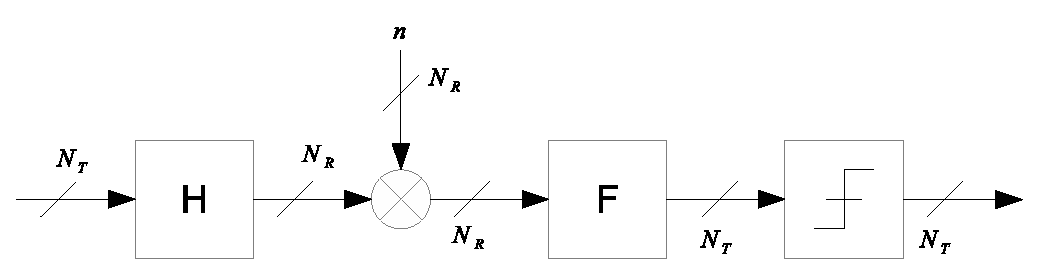
\includegraphics[width=1\textwidth]{linear_equalizer.eps} \\
	& \mathbf{H}\in\mathbb{C}^{N_R\times N_T};\qquad\mathbf{F}\in\mathbb{C}^{N_T\times N_R} \\
	& \mathbf{H}=
	\begin{pmatrix}
	0,2 & -0,2 \\
	0,1 & 0,4 \\
	1 & 0,2
	\end{pmatrix},\qquad\frac{\sigma_x^2}{\sigma_n^2}=10 \\
	& N_R>N_T\quad\rightarrow\quad \mathbf{F}=\left(\mathbf{H}^H\mathbf{H}\right)^{-1}\cdot\mathbf{H}^H\quad\rightarrow\quad\text{left Moore-Penrose pseudo-inverse} \\
	& \text{received signal: }r=\mathbf{FH}x+\mathbf{F}n\quad\rightarrow\quad\text{drawback: noise amplification} \\
	& r=\mathbf{FH}x+\mathbf{F}n=\underbrace{\left(\mathbf{H}^H\mathbf{H}\right)^{-1}\mathbf{H}^H\mathbf{H}}_{\mathbf{I}}x+\mathbf{F}n=x+\mathbf{F}n\quad\rightarrow\quad\text{no interference} \\
	& \rightarrow\quad\text{error signal: }e=\mathbf{F}n\quad\rightarrow\quad\phi_{ee}=ee^H=\mathbf{F}\underbrace{nn^H}_{\sigma_n^2\mathbf{I}}\mathbf{F}^H \\
	& \qquad\rightarrow\quad nn^H=\sigma_n^2\mathbf{I}\quad\text{white noise}
\end{align*}
\begin{align*}
	& \rightarrow\quad\phi_{ee}^{ZF}=\sigma_n^2\mathbf{FF}^H\quad\rightarrow\quad\phi_{ee}^{ZF}=\sigma_n^2
	\begin{pmatrix}
	1,13 & -0,94 \\
	-0,94 & 4,95
	\end{pmatrix} \\
	& \sigma_e^2=\tr\left(\phi_{ee}^{ZF}\right)=\sigma_n^2\left(1,13+4,95\right) \\
	& \Rightarrow\sigma_e^2=\sigma_n^2\cdot 6,1 \\
	& \text{Now determine $\mathbf{F}$ such that the error-variance is minimal!} \\
	& \rightarrow\quad\text{MMSE}\quad\rightarrow\quad\mathbf{F}=\left(\mathbf{H}^H\mathbf{H}+\frac{\sigma_n^2}{\sigma_x^2}\mathbf{I}\right)^{-1}\underbrace{\mathbf{H}^H}_{\substack{\text{matched}\\ \text{filter}}};\qquad\frac{\sigma_x^2}{\sigma_n^2}=10 \\
	& \Rightarrow\text{for low SNR: MMSE} \\
	& \Rightarrow\text{for high SNR: ZF} \\
	& \rightarrow\mathbf{F}=
	\begin{pmatrix}
	0,31 & -0,13 & 0,85 \\
	-0,77 & 1,25 & 0,086
	\end{pmatrix} \\
	& \rightarrow\text{from lecture notes:} \\
	& \quad\rightarrow\quad\phi_{ee}=\sigma_n^2\left(\mathbf{H}^H\mathbf{H}+\frac{\sigma_n^2}{\sigma_x^2}\mathbf{I}\right)^{-1}\quad\rightarrow\quad\phi_{ee}^{MMSE}=\sigma_n^2
	\begin{pmatrix}
	0,97 & -0,57 \\
	-6,57 & 3,28
	\end{pmatrix} \\
	& \quad\rightarrow\quad\text{total error variance = }\tr\left(\phi_{ee}\right) \\
	& \qquad\Rightarrow\quad\sigma_e^2=4,25\sigma_n^2 \\
	& \text{End-to-end channel: }\mathbf{K=FH=}
	\begin{pmatrix}
	0,9 & 0,06 \\
	0,06 & 0,67
	\end{pmatrix} \\
	& \text{residual interference in off-diagonal elements} \\
	&	\text{diagonal elements should be 1, but are not $\Rightarrow$ biased!} \\
	& \rightarrow\text{solution:}\quad\rightarrow\quad\text{remove bias by multiplying with }\mathbf{C}=
	\begin{pmatrix}
	\frac{1}{0,9} & 0 \\
	0 & \frac{1}{0,67}
	\end{pmatrix} \\
	& \rightarrow\mathbf{C}=
	\begin{pmatrix}
	1,11 & 0 \\
	0 & 1,49
	\end{pmatrix} \\
	& r'=\mathbf{C}r=
	\begin{pmatrix}
	1,11 & 0 \\
	0 & 1,49
	\end{pmatrix}
	\begin{pmatrix}
	0,9 & 0,06 \\
	0,06 & 0,67
	\end{pmatrix}x+
	\begin{pmatrix}
	1,11 & 0 \\
	0 & 1,49
	\end{pmatrix}\mathbf{F}n=\\
	& =
	\begin{pmatrix}
	1 & 0,07 \\
	0,09 & 1
	\end{pmatrix}x+
	\begin{pmatrix}
	1,11 & 0 \\
	0 & 1,49
	\end{pmatrix}\mathbf{F}n \\
	& \text{from lecture notes:} \\
	& \qquad\phi_{e'e'}=\sigma_x^2\left(\mathbf{I}+\left(\mathbf{C-I}\right)\mathbf{K}^H\mathbf{C}^H-\mathbf{CK}\right);\qquad\frac{\sigma_x^2}{\sigma_n^2}=10 \\
	& \qquad\Rightarrow\quad\sigma_x^2
	\begin{pmatrix}
	0,11 & -0,05 \\
	-0,05 & 0,49
	\end{pmatrix}=\sigma_n^2
	\begin{pmatrix}
	1,1 & -0,5 \\
	-0,5 & 4,5
	\end{pmatrix} \\
	& \qquad\rightarrow\quad\sigma_e'^2=\tr\left(\phi_{e'e'}\right)=6\sigma_n^2
\end{align*}
\begin{align*}
	& \text{Decision feedback:} \\
	& 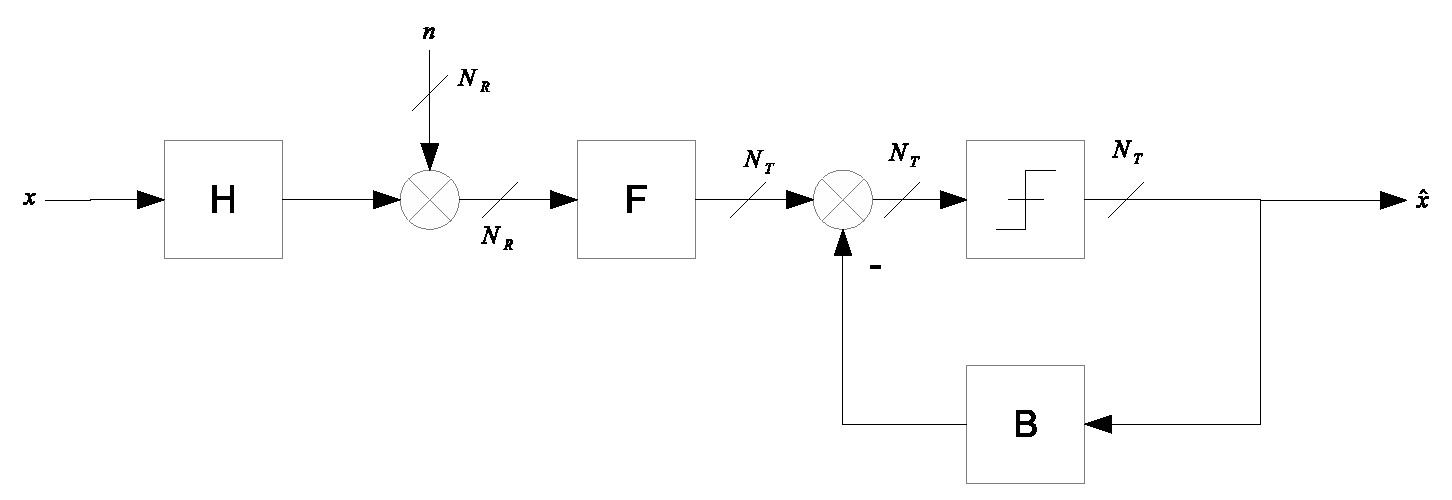
\includegraphics[width=1\textwidth]{decisionfeedback_equalizer.eps} \\
	& \mathbf{H}\in\mathbb{C}^{N_R\times N_T};\qquad\mathbf{F}\in\mathbb{C}^{N_T\times N_R} \\
	& \text{drawback: propagation of error when errors predictions are not accurate} \\
	& \left[\mathbf{L,D}\right]=???\left(\mathbf{H}^H\mathbf{H}\right)\quad\text{Cholesky factorization} \\
	& \mathbf{H}^H\mathbf{H}=
	\begin{pmatrix}
		1,03 & 0,2 \\
		0,2 & 0,24
	\end{pmatrix}\quad\rightarrow\quad\mathbf{L}=
	\begin{pmatrix}
	1 & 0 \\
	0,19 & 1
	\end{pmatrix},\qquad\mathbf{D}=
	\begin{pmatrix}
	1,03 & 0 \\
	0 & 0,2
	\end{pmatrix} \\
	& \qquad\text{feedforward filter:}\quad\mathbf{F=D}^{-1}\mathbf{C}^{-H}\mathbf{H}^H=
	\begin{pmatrix}
	0,23 & 0,02 & 0,96 \\
	-0,99 & 1,98 & 0,99
	\end{pmatrix} \\
	& \qquad\text{feedback filter:}\quad\mathbf{B=C-I}=
	\begin{pmatrix}
	1 & 0 \\
	0,19 & 1
	\end{pmatrix}-
	\begin{pmatrix}
	1 & 0 \\
	0 & 1
	\end{pmatrix}=
	\begin{pmatrix}
	0 & 0 \\
	0,19 & 0
	\end{pmatrix}
\end{align*}
\begin{align*}
	& \text{MMSE-DFE:} \\
	& \mathbf{LDL}^H=\mathbf{H}^H\mathbf{H}+\frac{\sigma_n^2}{\sigma_x^2}\mathbf{I}=
	\begin{pmatrix}
	1,15 & 0,2 \\
	0,2 & 0,34
	\end{pmatrix}
	\quad\rightarrow\quad\left(\mathbf{L,D}\right)\rightarrow \left(\mathbf{H}^H+\frac{\sigma_n^2}{\sigma_x^2}\mathbf{I}\right) \\
	& \rightarrow\quad\mathbf{L}=
	\begin{pmatrix}
	1 & 0 \\
	0,17 & 1
	\end{pmatrix},\quad\mathbf{D}=
	\begin{pmatrix}
	1,15 & 0 \\
	0 & 0,31
	\end{pmatrix} \\
	& \rightarrow\text{Feedforward filter: }\mathbf{F=C}\left|\mathbf{H}^H\mathbf{H}+\frac{\sigma_n^2}{\sigma_x^2}\mathbf{I}\right|^{-1}\mathbf{H}^H=
	\begin{pmatrix}
	0,19 & 0,21 & 1,13 \\
	0,005 & 0,15 & 0,48
	\end{pmatrix} \\
	& \rightarrow\text{Feedback filter: }\mathbf{B=L-I}=
	\begin{pmatrix}
	0 & 0 \\
	0,1739 & 0
	\end{pmatrix} \\
	& \rightarrow\text{Error covariance matrix: }\phi_{ee}=\sigma_n^2\mathbf{D}^{-1}=\sigma_n^2
	\begin{pmatrix}
	0,87 & 0 \\
	0 & 3,28
	\end{pmatrix} \\
	& \rightarrow\quad\sigma_e^2=\tr\left(\phi_{ee}\right)=4,15\sigma_n^2
\end{align*}

\end{document}